\documentclass[a4paper,12pt]{article}
%%%%%%%%%%%%%%%%%%%%%%%%%%%%%%%%%%%%%%%%%%%%%%%%%%%%%%%%%%%%%%%%%%%%%%%%%%%%%%%%%%%%%%%%%%%%%%%%%%%%%%%%%%%%%%%%%%%%%%%%%%%%%%%%%%%%%%%%%%%%%%%%%%%%%%%%%%%%%%%%%%%%%%%%%%%%%%%%%%%%%%%%%%%%%%%%%%%%%%%%%%%%%%%%%%%%%%%%%%%%%%%%%%%%%%%%%%%%%%%%%%%%%%%%%%%%
\usepackage{eurosym}
\usepackage{vmargin}
\usepackage{amsmath}
\usepackage{graphics}
\usepackage{epsfig}
\usepackage{subfigure}
\usepackage{fancyhdr}
\usepackage{listings}
\usepackage{framed}
\usepackage{graphicx}
\usepackage{amsmath}
\usepackage{chngpage}
%\usepackage{bigints}

%\setcounter{MaxMatrixCols}{10}

\begin{document}
	\large
	%%-
\section*{Bokeh Graphics with Jupyter Notebooks}
\begin{itemize}
\item Open up a Jupyter Notebook, and enter the following code in over three or four cells.
\item Run those cells. The output should come up on a new HTML page. (See next page).
\item The output graphic has some controls (pan , zoom, resize etc). Try these controls out.
\item Vary some of the values (width, either , title).
\end{itemize}
\begin{framed}
\begin{verbatim}
#Import library
from bokeh.charts import Bar, output_file, show 


#use output_file to visualize it in html file
#use output_notebook to visualize it in notebook

# create a simple data set
myData = {"y": [1, 2, 3, 4, 5]}

# Output to Line.HTML
output_file("lines.html", title="line plot example") 

# create a new line chat with a title and axis labels
p = Bar(myData, title="Simple Bar Chart Example",
     label='x', ylabel='values', 
     width=400, height=400)

# show the results
show(p)

\end{verbatim}
\end{framed}
\newpage
\begin{figure}[h!]
\centering
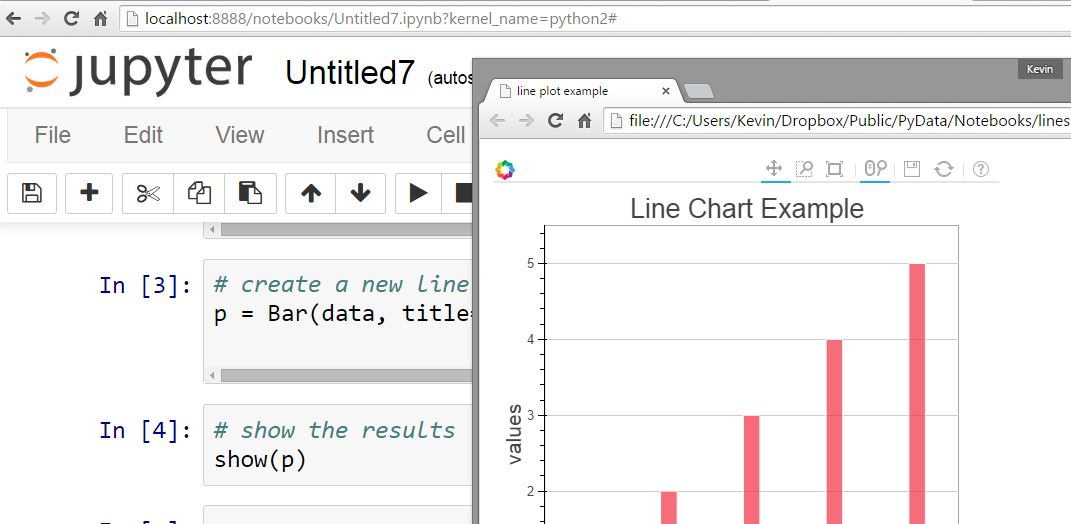
\includegraphics[width=0.9\linewidth]{images/OutPut}
\caption{Output}\vspace{0.5cm}
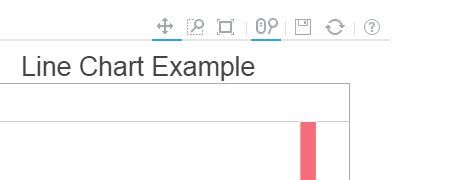
\includegraphics[width=0.8\linewidth]{images/TopRightCorner}
\caption{Controls}
\end{figure}

\end{document}